% To je predloga za poročila o domačih nalogah pri predmetih, katerih
% nosilec je Blaž Zupan. Seveda lahko tudi dodaš kakšen nov, zanimiv
% in uporaben element, ki ga v tej predlogi (še) ni. Več o LaTeX-u izveš na
% spletu, na primer na http://tobi.oetiker.ch/lshort/lshort.pdf.
%
% To predlogo lahko spremeniš v PDF dokument s pomočjo programa
% pdflatex, ki je del standardne instalacije LaTeX programov.

\documentclass[a4paper,11pt]{article}
\usepackage{a4wide}
\usepackage{fullpage}
\usepackage[utf8x]{inputenc}
\usepackage[slovene]{babel}
\selectlanguage{slovene}
\usepackage[toc,page]{appendix}
\usepackage[pdftex]{graphicx} % za slike
\usepackage{setspace}
\usepackage{color}
\definecolor{light-gray}{gray}{0.95}
\usepackage{listings} % za vključevanje kode
\usepackage{hyperref}
\renewcommand{\baselinestretch}{1.2} % za boljšo berljivost večji razmak
\renewcommand{\appendixpagename}{Priloge}

\lstset{ % nastavitve za izpis kode, sem lahko tudi kaj dodaš/spremeniš
language=Python,
basicstyle=\footnotesize,
basicstyle=\ttfamily\footnotesize\setstretch{1},
backgroundcolor=\color{light-gray},
}

\title{Filtri}
\author{David Rubin (david.rubin@student.um.si)}
\date{\today}

\begin{document}

\maketitle

\section{Zahteve naloge}

Filtru pravimo, da je stabilen, kadar se njegov impulzni odziv h(n) približuje vrednosti 0, ko gre n proti neskončnosti. V kontekstu ničel in polov Z transformacije to pomeni, da je filter stabilen samo takrat, kadar so vsi njegovi poli znotraj enotskega kroga v kompleksni ravnini Z.

Vaša naloga je izdelati svoj lasten ARMA filter vsaj petega reda in določiti koeficiente a in b tako, da bo filter nestabilen. Vsak študent mora imeti izbrane svoje unikatne koeficiente (očitne podobnosti in trivialne tranformacije koeficientov filtrov drugih študentov niso dovoljene). Za svoj filter odgovorite na naslednja vprašanja:  
\begin{enumerate}
 
\item Kako se glasi Z transformiranka vašega fitlra?
\item Kje v Z ravnini ležijo ničle vašega filtra?
\item Kje v Z ravnini ležijo poli vašega filtra?
\item Približno katere frekvence vaš filter prepušča in zakaj?
\item Približno katere frekvence vaš filter zapira in zakaj?
\item Kaj je treba narediti, da bo vaš filter postal stabilen in ohranil čim več originalnih frekvenčnih karakteristik?
\item Kako se s stabilizacijo filtra spremenijo koeficienti $a$?
\item Kako se s stabilizacijo filtra spremenijo koeficienti $b$?

\end{enumerate}
Z transformacijo filtra naredite ročno. Iskanje ničel polinomov, ki vam določajo ničle in pole filtra, lahko izvedete v različnih orodjih, ki omogočajo iskanje ničel.

\section{Poročilo}

Koda, s katero sem pridobil naslednje odgovore, je priložena k poročilu.
\begin{enumerate}
\item \textbf{Kako se glasi Z transformiranka vašega filtra?}

\[
H(z) = \frac{2 + 1z^{-1} - \frac{1}{9}z^{-2} + z^{-4} - \frac{7}{11}z^{-5} + 2z^{-6} }
		{\frac{3}{4} - z^{-1} + \frac{2}{3}z^{-2} - \frac{6}{13}z^{-3} - \frac{25}{29}z^{-4} - 3z^{-5} + \frac{3}{8}z^{-6}}
\]


\item \textbf{Kje v Z ravnini ležijo ničle vašega filtra?}

Glej sliko~\ref{nicle_before}.

\begin{figure}[htbp]
\begin{center}
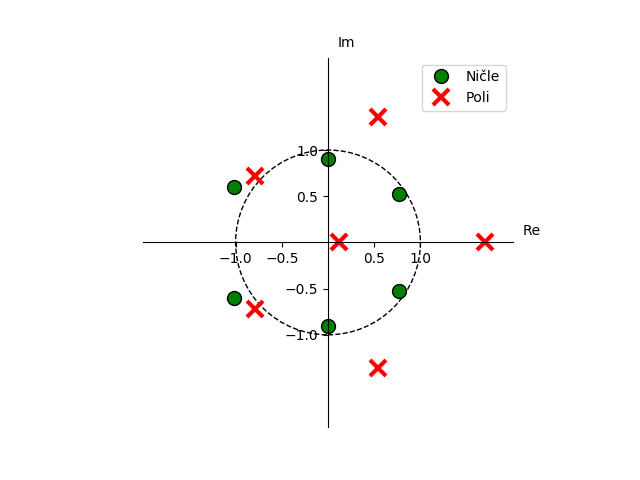
\includegraphics[scale=0.6]{images/zplane_before.png}
\caption{Ničle in poli filtra pred stabilizacijo.}
\label{nicle_before}
\end{center}
\end{figure}


\item \textbf{Kje v Z ravnini ležijo poli vašega filtra?}

Glej sliko~\ref{nicle_before}.


\item \textbf{Približno katere frekvence vaš filter prepušča in zakaj?}

Iz frekvenčnega odziva na sliki~\ref{refreq_before} lahko vidimo, da filter prepušča frekvence $0$ -- $0.1 \cdot f_{s}$, $0.3$ -- $0.4\cdot f_{s}$ in $0.6$ -- $0.8 \cdot f_{s}$.

\begin{figure}[htbp]
\begin{center}
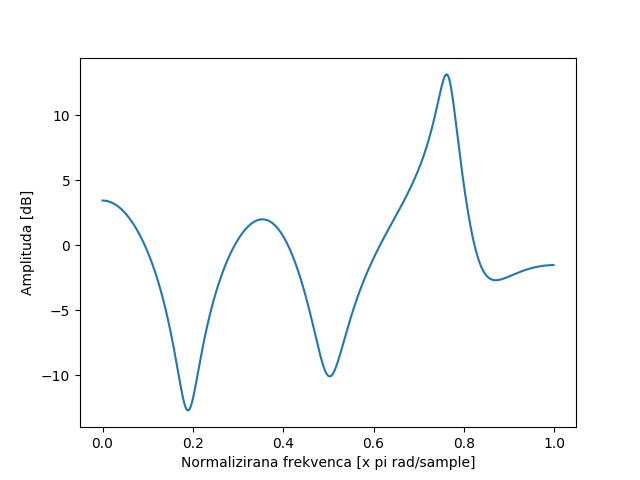
\includegraphics[scale=0.6]{images/freq-response_before.png}
\caption{Frekvenčni odziv nestabilnega filtra.}
\label{refreq_before}
\end{center}
\end{figure}


\item \textbf{Približno katere frekvence vaš filter zapira in zakaj?}

Na sliki~\ref{refreq_before} zopet lahko vidimo, da filter zapira frekvence $0.2 \cdot f_{s}$, $0.5 \cdot f_{s}$ in od $0.8 \cdot f_{s}$ dalje ($f_{s}$ predstavlja vzorčevalno frekvenco).


\item \textbf{Kaj je treba narediti, da bo vaš filter postal stabilen in ohranil čim več originalnih frekvenčnih karakteristik?}

Pole, ki so na sliki~\ref{nicle_before} zunaj enotskega kroga preslikamo znotraj kroga, tako da jih zamaknemo pod istim kotom in približno toliko kot so bili zunaj kroga so zatem znotraj kroga. Če z $p$ označimo prvotni pol, potem naš novi ocenjen pol $\tilde{p}$ pridobimo z naslednjo transformacijo:
\begin{equation}
\tilde{p} = \frac{1}{\bar{p}},
\end{equation}
kjer $\bar{p}$ predstavlja kompleksno konjugacijo.


\item \textbf{Kako se s stabilizacijo filtra spremenijo koeficienti $a$?}

Poli, ki so zunaj kroga se prestavijo v krog, tako dobimo nove koeficiente $a$:
\[
		1 + 0.172z^{-1} + 0.092z^{-2} - 0.194z^{-3} + 0.314z^{-4} - 0.276z^{-5} + 0.029z^{-6}
\]


\item \textbf{Kako se s stabilizacijo filtra spremenijo koeficienti $b$?}

Koeficienti $b$ ostanejo nespremenjeni.

\end{enumerate}

\begin{figure}[htbp]
\begin{center}
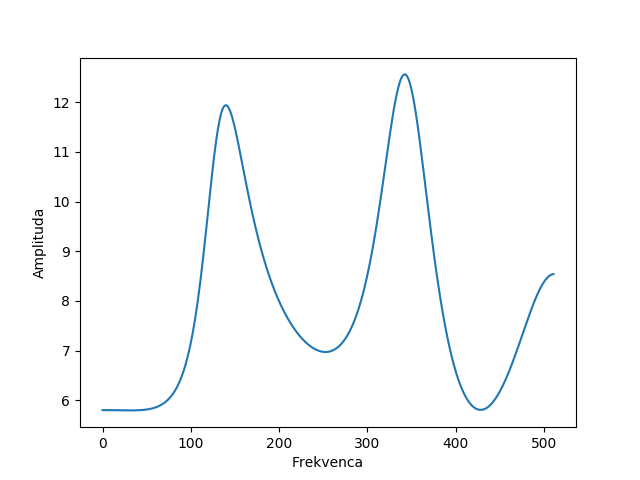
\includegraphics[scale=0.7]{images/freq-response_after.png}
\caption{Frekvenčni odziv stabilnega filtra.}
\label{refreq_after}
\end{center}
\end{figure}

\begin{figure}[htbp]
\begin{center}
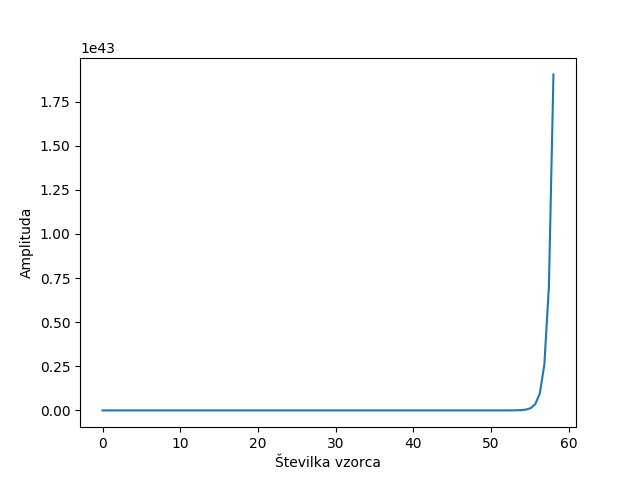
\includegraphics[scale=0.7]{images/impulse-response_before.png}
\caption{Impulzni odziv nestabilnega filtra.}
\label{reimp_before}
\end{center}
\end{figure}

\begin{figure}[htbp]
\begin{center}
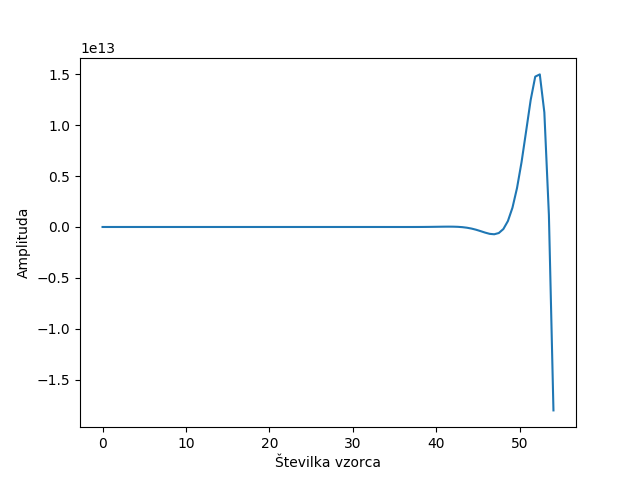
\includegraphics[scale=0.7]{images/impulse-response_after.png}
\caption{Impulzni odziv stabilnega filtra.}
\label{reimp_after}
\end{center}
\end{figure}


%\begin{figure}[htbp]
%\begin{center}
%\i%cludegraphics[scale=0.3]{slika-primer.png}
%\caption{Vsako sliko opremi s podnapisom, ki pove, kaj slika prikazuje.}
%\label{slika1}
%\end{center}
%\end{figure}

\end{document}
